\chapter{Énergie et hamiltonien}

\lectureoverview{Nous précisons d’abord la signification d’une symétrie active et
rappelons comment les translations et les rotations engendrent la quantité de mouvement et le moment cinétique.
La loi de conservation qui nous manque concerne l’énergie. Sa symétrie est la translation dans le temps,
et la grandeur conservée est le hamiltonien
\(H=\sum_i p_i\dot q_i-L\). La dérivation montre aussi précisément comment une dépendance explicite
en temps transfère de l’énergie entre un sous-système choisi et son
environnement.}

\section{Questions avant l’argument formel}

Nous approchons du minimum absolu de mécanique classique nécessaire pour aborder les
sujets qui suivent, même s’il reste beaucoup d’autres notions de mécanique qui méritent
d’être étudiées. Deux questions ont été posées avant le début de l’argument principal.

\begin{classroomqa}
  \audiencequestion{Quels ouvrages sont utiles après ce cours d’introduction ?
  \lecturetimestamp{00:00:36--00:02:13}}
  \lecturerresponse{L’ouvrage de référence avancé est celui d’Herbert
  Goldstein, \emph{Classical Mechanics}. Le livre de Cornelius Lanczos sur les
  principes variationnels de la mécanique est une autre source pertinente. Une
  liste de lecture pour le cours est plus utile que de prétendre qu’un seul enseignant peut passer en revue
  tous les ouvrages disponibles.}
\end{classroomqa}

La deuxième question évoque un épisode de l’histoire d’une mesure qui n’avait pas encore été élucidée.
En 2011, l’expérience OPERA avait signalé une arrivée apparemment précoce
de neutrinos envoyés du CERN au Gran Sasso. L’écart signalé
était plus court que la durée de l’impulsion de protons utilisée pour créer les neutrinos ; l’analyse temporelle
consistait donc à comparer les profils des impulsions plutôt qu’à identifier un
neutrino à l’émission puis à reconnaître la même particule à la détection.

\begin{classroomqa}
  \audiencequestion{Le résultat apparent de neutrinos plus rapides que la lumière avait-il
  été élucidé ?
  \lecturetimestamp{00:02:30--00:09:03}}
  \lecturerresponse{Aucune conclusion n’était alors justifiée. La forme de l’impulsion du faisceau,
  l’échauffement de la cible et la synchronisation exigeaient tous un examen technique approfondi. Une
  hypothèse spéculative portait sur le mouvement d’un satellite GPS : dans le référentiel du
  satellite, la source et le détecteur sont en mouvement pendant la propagation des signaux de synchronisation,
  ce qui produit des corrections de l’ordre de quelques dizaines de nanosecondes. Cette estimation
  était intéressante comme exercice d’ordre de grandeur, mais elle n’était pas présentée comme
  une explication crédible de l’expérience. La contraction de Lorentz ordinaire à
  la vitesse considérée était trop faible pour produire l’effet signalé. La bonne
  démarche consistait à attendre l’analyse expérimentale.}
\end{classroomqa}

\begin{figure}[htbp]
  \centering
  \includegraphics[width=0.78\textwidth]{lecture_05_figure_07.png}
  \caption{Schéma de synchronisation dans le référentiel du satellite, évoqué lors de la question historique
  sur la mesure des neutrinos.}
  \lectureframe{00:06:30}
\end{figure}

La discussion sur la synchronisation n’est pas nécessaire pour la mécanique qui suit. Elle est néanmoins utile
pour rappeler qu’une estimation d’ordre de grandeur plausible ne constitue pas en soi
une explication expérimentale établie.

\section{Symétrie active et choix du système}

Revenons au point qui était resté trop flou dans la discussion précédente : qu’est-ce précisément qu’une symétrie ? Considérons une particule sur une droite et
la transformation
\begin{equation}
  x\longrightarrow x+1.
  \label{eq:l5-shift-one}
\end{equation}
On peut l’interpréter de deux façons. Une transformation \emph{passive} renomme
les points de la droite. Un point autrefois appelé \(x=0\) peut désormais être appelé
\(x'=1\), mais la particule n’a pas bougé. Une transformation \emph{active}
conserve les étiquettes et déplace la particule elle-même de \(x\) à \(x+1\).
Seule la deuxième opération modifie sa position par rapport à un potentiel
externe.

\begin{figure}[htbp]
  \centering
  \includegraphics[width=0.82\textwidth]{lecture_05_figure_08.png}
  \caption{La règle \(x\mapsto x+1\), la droite de coordonnées fixe et un
  potentiel externe distinguent le mouvement actif du simple changement passif d’étiquettes.}
  \lectureframe{00:11:20}
\end{figure}

\begin{classroomqa}
  \audiencequestion{Si le déplacement de la particule modifie son énergie potentielle, est-ce
  parce que la source de ce potentiel est exclue du système ?
  \lecturetimestamp{00:12:19--00:14:18}}
  \lecturerresponse{Exactement. Parler d’``une particule dans un
  potentiel'' revient à diviser le monde entre la particule et un environnement massif,
  tel que la Terre, qui produit \(V(x)\). La Terre subit bien un recul, mais sa
  masse énorme rend celui-ci négligeable dans cette approximation. Déplacer
  la particule par rapport à la Terre supposée fixe peut modifier \(V\) ; translater la
  particule et la Terre ensemble ne le ferait pas.}
\end{classroomqa}

\begin{classroomqa}
  \audiencequestion{Dans l’exemple précédent de rotation, les vitesses
  changeaient-elles aussi, en plus des positions ?
  \lecturetimestamp{00:14:26--00:15:29}}
  \lecturerresponse{Oui. Une rotation active rigide agit sur toute l’histoire du système,
  et pas seulement sur une position à un instant donné. Les positions et les vecteurs vitesse
  subissent tous deux une rotation. En revanche, une translation constante appliquée à chaque
  instant modifie \(x\) mais laisse \(\dot x\) inchangée.}
\end{classroomqa}

La distinction entre système et environnement reviendra à deux reprises : lorsqu’un
appareil dépendant du temps échange de l’énergie avec un sous-système, puis lorsque
le frottement macroscopique dissimule l’énergie dans des mouvements microscopiques inobservés.

\section{Mouvements infinitésimaux dans l’espace des configurations}

Une configuration d’un système mécanique général est un point de l’espace des
coordonnées généralisées \(q_i\). Une transformation infinitésimale active déplace
chaque configuration possible vers une configuration voisine. On écrit
\begin{equation}
  \delta q_i=\epsilon f_i(q),
  \label{eq:l5-general-transformation}
\end{equation}
où les fonctions \(f_i\) définissent un champ de déplacement donné dans
l’espace des configurations. Elles peuvent dépendre de toutes les coordonnées, et certaines peuvent
être nulles. Le facteur commun \(\epsilon\) est petit ; il sépare l’amplitude du
pas de la forme de la transformation.

\begin{figure}[htbp]
  \centering
  \includegraphics[width=0.75\textwidth]{lecture_05_figure_09.png}
  \caption{Un vecteur déplacement attaché à chaque point de l’espace des configurations.}
  \lectureframe{00:16:50}
\end{figure}

\begin{figure}[htbp]
  \centering
  \includegraphics[width=0.80\textwidth]{lecture_05_figure_10.png}
  \caption{La transformation infinitésimale dépendant des coordonnées
  \(\delta q_i=\epsilon f_i(q)\).}
  \lectureframe{00:18:00}
\end{figure}

La règle elle-même ne dépend pas explicitement du temps. Son action sur les vitesses est donc
\begin{equation}
  \delta\dot q_i=\frac{d}{dt}(\delta q_i)
  =\epsilon\sum_j\frac{\partial f_i}{\partial q_j}\dot q_j.
  \label{eq:l5-velocity-variation}
\end{equation}
Pour une translation, \(f_x=1\), donc \(\delta\dot x=0\). Pour une rotation,
\(f_i\) dépend de la position, et la vitesse est modifiée.

\begin{classroomqa}
  \audiencequestion{Le dernier petit facteur dans
  \(\delta q_i=\epsilon f_i(q)\) est-il la même constante en tout point ?
  \lecturetimestamp{00:19:58--00:20:51}}
  \lecturerresponse{Oui. L’unique constante \(\epsilon\) est un artifice de calcul
  qui fait que toutes les variations des coordonnées sont du premier ordre par rapport à la même
  petite quantité. Ce sont les fonctions \(f_i(q)\), et non \(\epsilon\), qui contiennent la dépendance spatiale
  et qui ne sont pas nécessairement petites.}
\end{classroomqa}

\section{Qu’est-ce qui fait de la transformation une symétrie ?}

Une transformation active modifie généralement l’énergie potentielle. Elle peut aussi
modifier l’énergie cinétique. En coordonnées curvilignes, le terme cinétique prend
la forme
\begin{equation}
  T=\frac12\sum_{i,j}g_{ij}(q)\dot q_i\dot q_j,
  \label{eq:l5-kinetic-metric}
\end{equation}
de sorte qu’un déplacement dans l’espace des configurations peut en modifier les coefficients. Le terme familier
\(r^2\dot\theta^2\) en coordonnées polaires en est l’exemple le plus simple.

Une transformation est une symétrie ici lorsque le lagrangien \emph{tout entier} ne subit
aucune variation du premier ordre,
\begin{equation}
  \delta L=O(\epsilon^2),
  \label{eq:l5-symmetry-condition}
\end{equation}
et cette condition doit être satisfaite en tout point de l’espace des configurations, et pas seulement pour la
configuration occupée par une solution particulière.

Par exemple, sous la transformation \(x\mapsto x+\epsilon\),
\begin{equation}
  \delta V=\frac{\partial V}{\partial x}\epsilon.
  \label{eq:l5-potential-variation}
\end{equation}
Si cette variation s’annule pour tout \(x\) possible, alors
\(\partial V/\partial x=0\) : le potentiel ne dépend pas de \(x\). S’il reste inchangé sous les translations dans toutes les directions de l’espace, il est constant.

\begin{figure}[htbp]
  \centering
  \includegraphics[width=0.80\textwidth]{lecture_05_figure_11.png}
  \caption{Une translation selon \(x\) testée pour un potentiel \(V(y)\) indépendant de \(x\).}
  \lectureframe{00:23:40}
\end{figure}

Pour une famille régulière à un paramètre, l’annulation de la variation du premier ordre en tout point permet de composer les pas infinitésimaux pour obtenir une symétrie finie.

\begin{classroomqa}
  \audiencequestion{L’énergie cinétique et l’énergie potentielle doivent-elles rester invariantes
  séparément ?
  \lecturetimestamp{00:24:44--00:25:33}}
  \lecturerresponse{Non. Seul le lagrangien total doit être invariant. Certains
  lagrangiens contiennent des termes mixtes coordonnée--vitesse et ne permettent pas une
  séparation utile en \(T\) et \(V\) ; la question de l’invariance séparée peut donc même
  ne pas avoir de sens.}
\end{classroomqa}

\begin{classroomqa}
  \audiencequestion{L’expression ``aucune variation'' signifie-t-elle une absence exacte de variation, ou seulement une
  variation assez faible pour être négligée ?
  \lecturetimestamp{00:25:34--00:28:59}}
  \lecturerresponse{Pour une transformation infinitésimale, elle signifie qu’il n’y a aucun terme
  proportionnel à \(\epsilon\). Les termes d’ordre \(\epsilon^2\) sont négligés dans
  le calcul local. Puisque la condition du premier ordre est satisfaite partout
  le long de l’orbite à un paramètre, la répétition du pas local donne l’invariance finie.}
\end{classroomqa}

\section{Quantité de mouvement et moment cinétique retrouvés}

Pour les symétries ponctuelles exactes et indépendantes du temps considérées ici, le résultat
établi précédemment est
\begin{equation}
  Q=\sum_i p_i f_i(q),
  \qquad
  p_i=\frac{\partial L}{\partial\dot q_i},
  \qquad
  \dot Q=0.
  \label{eq:l5-noether-charge}
\end{equation}
Le facteur \(\epsilon\) n’intervient pas dans \(Q\) ; il mesure seulement la distance parcourue
le long de l’orbite de symétrie.

\begin{figure}[htbp]
  \centering
  \includegraphics[width=0.82\textwidth]{lecture_05_figure_12.png}
  \caption{Le déplacement infinitésimal général et sa charge de Noether conservée.}
  \lectureframe{00:30:00}
\end{figure}

Pour une translation selon \(x\), \(f_x=1\) et \(Q=p_x\). L’invariance complète par translation
implique la conservation des trois composantes de la quantité de mouvement. Pour plusieurs
particules en interaction, la symétrie translate toutes les particules ensemble, de sorte que
\begin{equation}
  \mathbf P=\sum_a\mathbf p_a
  \label{eq:l5-total-momentum}
\end{equation}
est conservée lorsque les interactions ne dépendent que des positions relatives. Déplacer
une particule par rapport aux autres ne constitue pas la symétrie.

\begin{figure}[htbp]
  \centering
  \includegraphics[width=0.80\textwidth]{lecture_05_figure_13.png}
  \caption{Une translation commune entraîne la conservation de la quantité de mouvement totale,
  composante par composante.}
  \lectureframe{00:32:50}
\end{figure}

Pour une rotation infinitésimale dans le plan \(x\)-\(y\), choisissons l’orientation
\begin{equation}
  \delta x=-y\epsilon,
  \qquad
  \delta y=x\epsilon.
  \label{eq:l5-planar-rotation}
\end{equation}
Le rayon est conservé car
\begin{equation}
  \delta(x^2+y^2)
  =2x\delta x+2y\delta y=0.
  \label{eq:l5-radius-invariance}
\end{equation}

\begin{figure}[htbp]
  \centering
  \includegraphics[width=0.76\textwidth]{lecture_05_figure_14.png}
  \caption{Géométrie et formule en coordonnées d’une rotation plane infinitésimale.}
  \lectureframe{00:35:05}
\end{figure}

La dérivation de l’équation ~\eqref{eq:l5-planar-rotation} fait également tourner les vitesses.
Ainsi, \(\dot x^2+\dot y^2\) est invariant et un potentiel central
\(V(\sqrt{x^2+y^2})\) laisse le lagrangien complet inchangé. La charge est
\begin{equation}
  Q=-yp_x+xp_y=(\mathbf r\times\mathbf p)_z.
  \label{eq:l5-angular-charge}
\end{equation}

\begin{figure}[htbp]
  \centering
  \includegraphics[width=0.76\textwidth]{lecture_05_figure_15.png}
  \caption{La charge de Noether associée à la rotation, la composante selon \(z\) du moment cinétique.}
  \lectureframe{00:38:50}
\end{figure}

Les rotations dans les autres plans de coordonnées donnent les composantes restantes. Pour
plusieurs particules, le vecteur conservé est
\begin{equation}
  \mathbf J=\sum_a\mathbf r_a\times\mathbf p_a.
  \label{eq:l5-total-angular-momentum}
\end{equation}
Une planète soumise au potentiel central d’une étoile en est l’exemple fondamental : l’invariance sous toutes
les rotations implique la conservation de toutes les composantes du moment cinétique.

\begin{classroomqa}
  \audiencequestion{Que se passe-t-il au niveau d’une pointe, lorsque la dérivée d’un côté
  diffère de celle de l’autre côté ?
  \lecturetimestamp{00:42:25--00:44:21}}
  \lecturerresponse{C’est une réserve légitime. Le présent
  argument suppose des fonctions différentiables dont les dérivées sont uniques. Un
  équilibre instable, tel qu’un objet en équilibre au sommet d’un maximum lisse, ne pose
  pas de problème : la dérivée y existe et s’annule. Une pointe au sens strict exige un traitement modifié.}
\end{classroomqa}

\begin{classroomqa}
  \audiencequestion{Si le paramètre de transformation est indépendant du temps,
  pourquoi une rotation modifie-t-elle les vitesses ?
  \lecturetimestamp{00:44:23--00:45:23}}
  \lecturerresponse{Le paramètre est constant, mais le champ de déplacement dépend des
  coordonnées. La règle générale est
  \(\delta\dot q_i=d(\delta q_i)/dt\). Une translation a un \(\delta x\) constant,
  tandis que, pour une rotation, \(\delta x=-y\epsilon\) et par conséquent
  \(\delta\dot x=-\dot y\epsilon\).}
\end{classroomqa}

\section{Au-delà de la forme élémentaire énergie cinétique moins énergie potentielle}

En coordonnées cartésiennes, pour des particules ordinaires non relativistes sans
champ magnétique, \(L=T-V\). Des coordonnées plus générales conduisent à la forme quadratique de l’équation ~\eqref{eq:l5-kinetic-metric}. Un champ magnétique introduit un terme
linéaire en vitesse, schématiquement \(\mathbf A(q)\cdot\dot{\mathbf q}\), qui
mêle coordonnées et vitesses. Dans ce cas, mieux vaut traiter
\(L(q,\dot q,t)\) comme une seule fonction que de vouloir ranger chaque terme dans les catégories conventionnelles
d’énergie cinétique et d’énergie potentielle.

\begin{figure}[htbp]
  \centering
  \includegraphics[width=0.80\textwidth]{lecture_05_figure_16.png}
  \caption{Un terme cinétique quadratique général dépendant des coordonnées, à côté d’un
  potentiel qui ne dépend que des coordonnées.}
  \lectureframe{00:47:20}
\end{figure}

\begin{classroomqa}
  \audiencequestion{Pourquoi un lagrangien peut-il ne pas se séparer nettement en
  énergie cinétique et énergie potentielle, et est-il toujours défini comme \(T-V\) ?
  \lecturetimestamp{00:45:26--00:48:13}}
  \lecturerresponse{L’obstacle peut venir de coordonnées curvilignes ou
  d’interactions réellement dépendantes de la vitesse, comme le magnétisme. Ce n’est que lorsque
  le lagrangien est constitué d’une forme quadratique en les vitesses moins une fonction qui ne dépend que des coordonnées
  que l’on désigne ces termes par \(T\) et \(V\). Sinon, le lagrangien
  reste une fonction parfaitement valable de \(q\) et \(\dot q\), mais cette décomposition
  n’est pas utile. La définition générale correcte de l’énergie viendra
  du hamiltonien.}
\end{classroomqa}

\begin{classroomqa}
  \audiencequestion{L’exemple de la chaîne suspendue lors de la première séance était-il
  une application du principe de moindre action ?
  \lecturetimestamp{00:48:15--00:49:45}}
  \lecturerresponse{Il s’agissait d’un problème d’équilibre régi par l’énergie minimale,
  et non d’une histoire sélectionnée par une action stationnaire. Pour une solution statique d’un système ordinaire \(T-V\), \(\dot p_i=0\) et l’équation d’Euler--Lagrange se réduit à \(\partial V/\partial q_i=0\), la condition pour que le potentiel soit
  stationnaire.}
\end{classroomqa}

La quantité de mouvement et le moment cinétique sont désormais reliés aux symétries spatiales. La
grandeur qui manque de façon évidente est l’énergie.

\section{Invariance par translation dans le temps}

Imaginons une expérience qui commence à \(t_0\), se termine à \(t_1\) et produit un
résultat. Répétons la même préparation plus tard, en commençant à
\(t_0+\Delta t\) et en terminant à \(t_1+\Delta t\). Si le résultat ne change pas,
le système est invariant sous une translation active dans le temps.

\begin{figure}[htbp]
  \centering
  \includegraphics[width=0.82\textwidth]{lecture_05_figure_17.png}
  \caption{Une expérience et sa copie translatée dans le temps, représentées comme des histoires dans l’espace des configurations.}
  \lectureframe{00:52:45}
\end{figure}

Une particule chargée entre les plaques d’un condensateur illustre la rupture de cette
symétrie. Si la charge des plaques est fixe, la même expérience peut être réalisée
à n’importe quel moment. Si un générateur externe charge les plaques de façon continue,
la particule subit un champ électrique différent selon le moment où elle est libérée.
La particule constitue alors un sous-système soumis à une excitation explicite.

\begin{figure}[htbp]
  \centering
  \includegraphics[width=0.82\textwidth]{lecture_05_figure_18.png}
  \caption{Comparaison entre des plaques de condensateur fixes et des plaques dont la charge varie sous l’effet d’une source externe, à côté du schéma de translation temporelle.}
  \lectureframe{00:54:45}
\end{figure}

Le même phénomène apparaît pour un oscillateur,
\begin{equation}
  L=\frac12m\dot x^2-\frac12k(t)x^2.
  \label{eq:l5-driven-oscillator}
\end{equation}
Un champ électrique ou magnétique externe pourrait modifier lentement le matériau et
par conséquent sa constante de raideur effective. Si \(k\) varie, décaler l’expérience de l’oscillateur dans le temps en modifie le résultat.

\begin{figure}[htbp]
  \centering
  \includegraphics[width=0.78\textwidth]{lecture_05_figure_19.png}
  \caption{Termes cinétique et potentiel de l’oscillateur lors de la discussion
  d’une constante de raideur dépendant du temps.}
  \lectureframe{00:56:45}
\end{figure}

Si l’appareil qui modifie \(k\) est inclus dans le système, on peut à nouveau translater dans le temps l’expérience complète, désormais fermée, et son énergie totale se conserve.
La non-conservation apparente correspond à un échange d’énergie à travers une frontière que nous avons choisie.

Pendant la pause, le petit paramètre de transformation a été renommé
\(\epsilon\), pour éviter l’expression visuellement déroutante
\(\delta x=\delta\). Une suggestion de lecture sur Emmy Noether a
également été signalée pour la liste de lecture commune.

\begin{classroomqa}
  \audiencequestion{Si le lagrangien n’est pas donné sous la forme \(T-V\), d’où vient-il ?
  \lecturetimestamp{01:00:17--01:02:24}}
  \lecturerresponse{On peut l’inférer à partir d’expériences, le reconstruire à partir
  d’équations du mouvement connues, le conjecturer à partir de symétries et d’autres principes
  théoriques, ou le trouver par tâtonnements. Une fois \(L(q,\dot q,t)\) donné,
  le calcul d’Euler--Lagrange permet d’obtenir les équations du mouvement. L’argument formel
  ne nous oblige pas à déterminer d’abord son origine.}
\end{classroomqa}

Le critère opérationnel de l’invariance par translation dans le temps est maintenant immédiat. Si
la connaissance de \(q\) et de \(\dot q\) suffit à déterminer \(L\), sans qu’il soit nécessaire de connaître aussi
le temps indiqué par l’horloge, alors
\begin{equation}
  \frac{\partial L}{\partial t}=0.
  \label{eq:l5-no-explicit-time}
\end{equation}
Cela ne signifie pas que \(L(q(t),\dot q(t))\) est constant au cours du mouvement. Cela
signifie seulement qu’il n’y a pas de dépendance temporelle autre que celle portée par les coordonnées et les vitesses qui évoluent.

Un lourd haltère en rotation fournit un autre exemple de système soumis à une excitation. Si son mouvement imposé crée un potentiel gravitationnel variable dans le temps pour une particule test légère, le lagrangien de cette particule dépend explicitement du temps. Traiter
l’haltère comme un système dynamique agrandirait le système et éliminerait cette
variation temporelle externe.

\begin{figure}[htbp]
  \centering
  \includegraphics[width=0.80\textwidth]{lecture_05_figure_20.png}
  \caption{Un haltère en rotation imposée agit comme une source externe dépendant du temps
  pour une particule plus légère.}
  \lectureframe{01:06:25}
\end{figure}

\section{Dérivation du hamiltonien}

Supposons que nous ne connaissions pas la formule de l’énergie et que nous conjecturions que le
lagrangien lui-même est conservé. Pour le vérifier directement, dérivons-le
le long d’une trajectoire réelle. Commençons, pour simplifier, par le cas sans dépendance explicite en temps :
\begin{equation}
  \frac{dL}{dt}
  =\sum_i\left(
    \frac{\partial L}{\partial q_i}\dot q_i
    +\frac{\partial L}{\partial\dot q_i}\ddot q_i
  \right).
  \label{eq:l5-chain-rule-no-time}
\end{equation}

\begin{figure}[htbp]
  \centering
  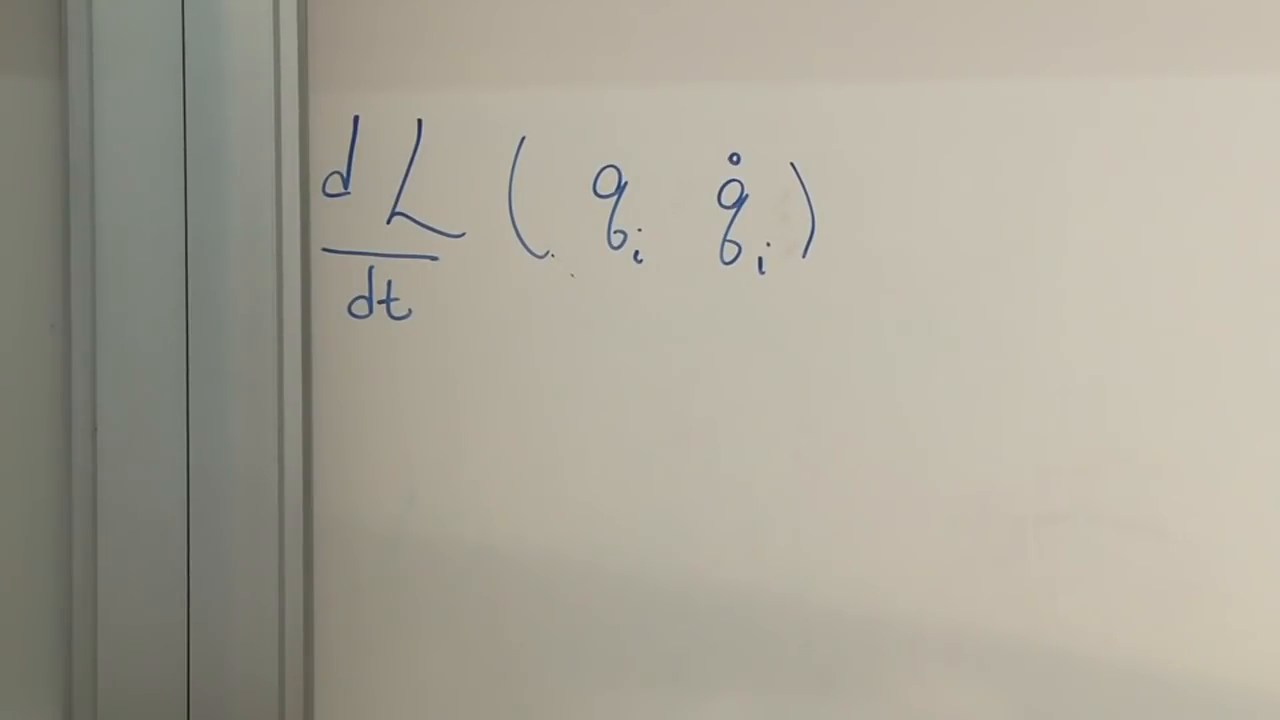
\includegraphics[width=0.72\textwidth]{lecture_05_figure_02.png}
  \caption{Début de la dérivation de \(L(q_i,\dot q_i)\) le long de la
  trajectoire.}
  \lectureframe{01:08:51}
\end{figure}

\begin{classroomqa}
  \audiencequestion{Ne manque-t-il pas une somme dans l’expression obtenue par la règle de dérivation en chaîne ?
  \lecturetimestamp{01:10:39--01:11:05}}
  \lecturerresponse{Oui. Chaque coordonnée et chaque vitesse peut modifier le
  lagrangien, donc les deux termes sont sommés sur \(i\).}
\end{classroomqa}

Utilisons la quantité de mouvement canonique et l’équation d’Euler--Lagrange,
\begin{equation}
  p_i=\frac{\partial L}{\partial\dot q_i},
  \qquad
  \dot p_i=\frac{\partial L}{\partial q_i}.
  \label{eq:l5-p-and-pdot}
\end{equation}
L’équation ~\eqref{eq:l5-chain-rule-no-time} devient
\begin{align}
  \frac{dL}{dt}
  &=\sum_i(\dot p_i\dot q_i+p_i\ddot q_i)
  \notag\\
  &=\frac{d}{dt}\sum_i p_i\dot q_i.
  \label{eq:l5-product-rule}
\end{align}
La ``magie'' n’est que la règle du produit.

\begin{figure}[htbp]
  \centering
  \includegraphics[width=0.84\textwidth]{lecture_05_figure_21.png}
  \caption{La règle de dérivation en chaîne, transformée à l’aide des équations du mouvement en la
  dérivée de \(\sum_i p_i\dot q_i\).}
  \lectureframe{01:13:45}
\end{figure}

\begin{classroomqa}
  \audiencequestion{Le dernier \(q_i\) dans le produit doit-il porter un point ou
  deux ?
  \lecturetimestamp{01:14:31--01:15:32}}
  \lecturerresponse{Dans le produit, il s’agit de \(p_i\dot q_i\), avec un seul point.
  La dérivation du produit donne
  \(\dot p_i\dot q_i+p_i\ddot q_i\), ce qui explique les deux points dans le
  deuxième terme développé.}
\end{classroomqa}

La soustraction des deux dérivées donne une combinaison conservée. Par convention
historique, on choisit son opposé et on l’appelle le hamiltonien :
\begin{equation}
  H=\sum_i p_i\dot q_i-L.
  \label{eq:l5-hamiltonian-definition}
\end{equation}

\begin{figure}[htbp]
  \centering
  \includegraphics[width=0.80\textwidth]{lecture_05_figure_22.png}
  \caption{La combinaison conservée \(L-\sum_i p_i\dot q_i=-H\) et la définition du hamiltonien.}
  \lectureframe{01:18:05}
\end{figure}

Pour une particule dans un potentiel,
\begin{equation}
  L=\frac12m\dot x^2-V(x),
  \qquad p=m\dot x.
  \label{eq:l5-particle-lagrangian}
\end{equation}
On obtient donc
\begin{align}
  H&=p\dot x-L
  \notag\\
   &=m\dot x^2-\left(\frac12m\dot x^2-V(x)\right)
  \notag\\
   &=\frac12m\dot x^2+V(x)=T+V.
  \label{eq:l5-particle-energy}
\end{align}

\begin{figure}[htbp]
  \centering
  \includegraphics[width=0.86\textwidth]{lecture_05_figure_23.png}
  \caption{Le hamiltonien d’une particule dans un potentiel se réduit à la somme familière
  de l’énergie cinétique et de l’énergie potentielle.}
  \lectureframe{01:20:50}
\end{figure}

La dérivation ne supposait aucune forme particulière pour \(L\). Ainsi,
l’équation ~\eqref{eq:l5-hamiltonian-definition}, plutôt que \(T+V\), constitue la définition générale
de l’énergie dans ce formalisme.

\section{Dépendance explicite en temps et échange d’énergie}

Rétablissons la dépendance explicite en temps dans la règle de dérivation en chaîne :
\begin{equation}
  \frac{dL}{dt}
  =\sum_i\left(
    \frac{\partial L}{\partial q_i}\dot q_i
    +\frac{\partial L}{\partial\dot q_i}\ddot q_i
  \right)
  +\frac{\partial L}{\partial t}.
  \label{eq:l5-full-chain-rule}
\end{equation}
Le membre de gauche est la dérivée totale le long du mouvement. La dérivée partielle finale
est calculée à \(q\) et \(\dot q\) fixés et porte uniquement sur les paramètres qui varient extérieurement. En répétant la même étape fondée sur la règle du produit, on obtient
\begin{equation}
  \boxed{\frac{dH}{dt}=-\frac{\partial L}{\partial t}}.
  \label{eq:l5-hamiltonian-time}
\end{equation}

\begin{figure}[htbp]
  \centering
  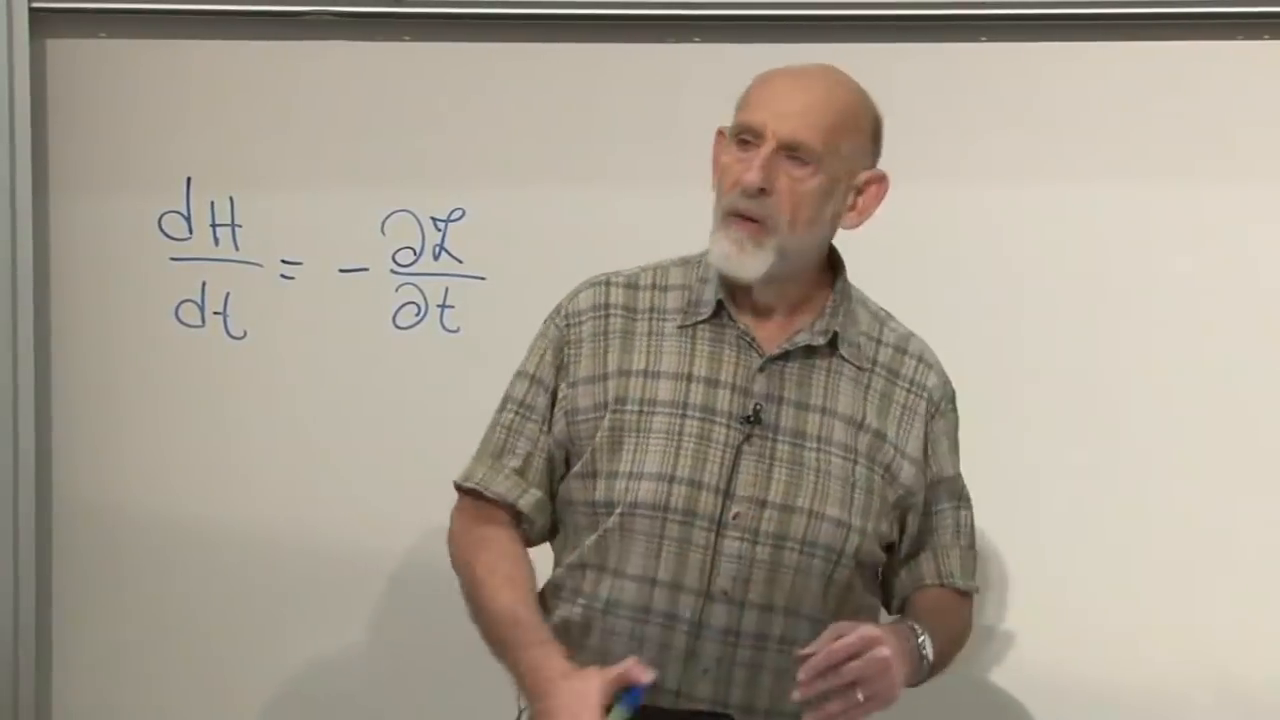
\includegraphics[width=0.70\textwidth]{lecture_05_figure_04.png}
  \caption{Le hamiltonien ne varie qu’en raison de la dépendance explicite en temps du lagrangien.}
  \lectureframe{01:37:22}
\end{figure}

Pour l’oscillateur soumis à une excitation de l’équation ~\eqref{eq:l5-driven-oscillator},
\begin{equation}
  \frac{\partial L}{\partial t}
  =-\frac12\dot k(t)x^2,
  \qquad
  \dot H=\frac12\dot k(t)x^2.
  \label{eq:l5-driven-energy-rate}
\end{equation}
En \(x=0\), le taux instantané s’annule ; en dehors de l’origine, la variation de la constante de
raideur fournit un travail à un taux proportionnel à \(x^2\dot k\).

\begin{classroomqa}
  \audiencequestion{Si l’énergie n’est pas conservée, sa définition est-elle la dérivée temporelle
  du hamiltonien ?
  \lecturetimestamp{01:27:11--01:28:04}}
  \lecturerresponse{Non. L’énergie est \(H\). Sa dérivée indique comment
  cette énergie varie. Lorsque le lagrangien prend la forme familière, \(H=T+V\) ;
  sinon, l’équation ~\eqref{eq:l5-hamiltonian-definition} en donne
  la définition. Agrandir le système pour y inclure le dispositif qui impose l’évolution rétablit
  la conservation du hamiltonien total.}
\end{classroomqa}

\begin{classroomqa}
  \audiencequestion{Qu’en est-il de l’observateur évoqué précédemment sur un
  manège en rotation, pour lequel apparaissaient les termes centrifuge et de Coriolis ?
  \lecturetimestamp{01:28:08--01:29:52}}
  \lecturerresponse{Un système de coordonnées en rotation uniforme constitue un
  changement de variables dépendant du temps, et non une symétrie spatiale fixe ni une
  simple translation dans le temps. Son lagrangien transformé peut servir à
  construire un hamiltonien, mais mieux vaut reporter ce calcul distinct
  à l’étude des forces magnétiques, car l’algèbre a une forme étroitement
  apparentée.}
\end{classroomqa}

\section{La boîte à outils lagrangienne en un coup d’œil}

On peut maintenant résumer toute la structure sous forme d’un ensemble compact de formules :
\begin{align}
  L&=L(q_i,\dot q_i,t),
  \notag\\
  p_i&=\frac{\partial L}{\partial\dot q_i},
  \qquad
  \dot p_i=\frac{\partial L}{\partial q_i},
  \notag\\
  \delta q_i&=\epsilon f_i(q)
  \quad\Longrightarrow\quad
  Q=\sum_i p_i f_i(q),\quad \dot Q=0,
  \notag\\
  H&=\sum_i p_i\dot q_i-L,
  \qquad
  \dot H=-\frac{\partial L}{\partial t}.
  \label{eq:l5-toolkit}
\end{align}

\begin{figure}[htbp]
  \centering
  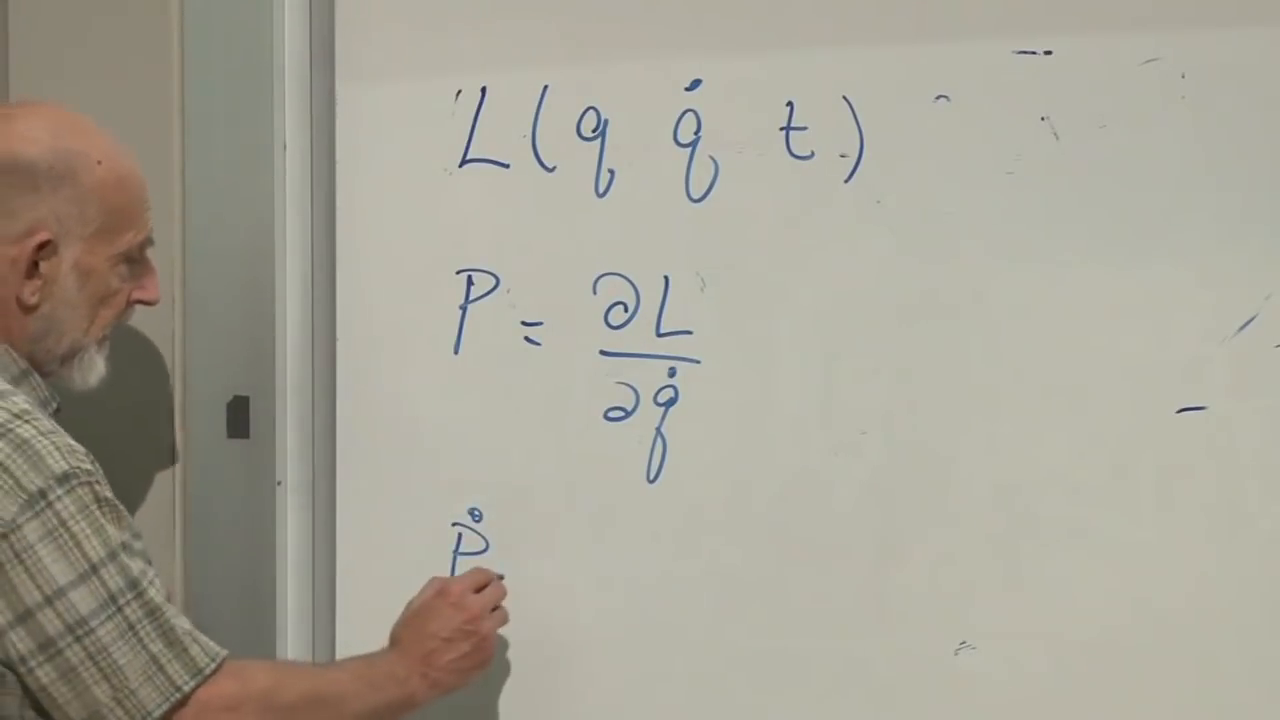
\includegraphics[width=0.66\textwidth]{lecture_05_figure_03.png}
  \caption{Le récapitulatif au tableau commence par \(L(q,\dot q,t)\), la quantité de mouvement canonique
  et l’équation d’Euler--Lagrange.}
  \lectureframe{01:31:37}
\end{figure}

Ces formules comprennent une définition, les équations du mouvement, la charge d’une
symétrie continue ordinaire et la charge associée à la translation dans le temps. Il y a
peu d’astuces ; l’essentiel est de savoir les redémontrer plutôt que de
mémoriser des expressions sans lien entre elles.

\section{Pourquoi utiliser la mécanique lagrangienne ou hamiltonienne ?}

\begin{classroomqa}
  \audiencequestion{Peut-on décrire la mécanique aussi bien avec \(L\) qu’avec \(H\),
  et pourquoi choisir l’une ou l’autre formulation ?
  \lecturetimestamp{01:37:16--01:39:18}}
  \lecturerresponse{Elles sont équivalentes lorsque la transformation de Legendre est
  régulière, mais elles mettent en avant des structures différentes. La formulation lagrangienne part
  naturellement du principe d’action stationnaire. La mécanique hamiltonienne est plus abstraite
  au début, mais ses équations sont simples et elle devient centrale en mécanique
  quantique. Le hamiltonien est l’énergie, mais son rôle dépasse largement la seule
  loi de conservation.}
\end{classroomqa}

\begin{classroomqa}
  \audiencequestion{Newton connaissait-il la forme hamiltonienne de la conservation
  de l’énergie ?
  \lecturetimestamp{01:39:29--01:39:56}}
  \lecturerresponse{Pas sous cette forme, d’après ce que l’on peut déduire des sources historiques.
  Le cadre formulé par Newton reposait sur la loi de force \(F=ma\).}
\end{classroomqa}

\begin{classroomqa}
  \audiencequestion{Pourquoi tout système physique devrait-il posséder un lagrangien ?
  Est-ce simplement un fait expérimental ?
  \lecturetimestamp{01:39:57--01:42:37}}
  \lecturerresponse{Pour les systèmes fermés considérés ici, c’est un fait empirique,
  et cela découle aussi de la description quantique plus fondamentale. On peut inventer des équations
  différentielles mathématiquement cohérentes qui ne sont pas des équations d’Euler--Lagrange. Par exemple, \(\dot x=-x\) se résout parfaitement,
  mais, en tant que loi fondamentale à une coordonnée pour un système fermé, elle présente le caractère dissipatif
  d’une perte d’information. La mécanique classique ne précède pas logiquement
  la mécanique quantique ; sa structure fondamentale lui vient de la mécanique
  quantique. Il faudra attendre pour en connaître la raison détaillée.}
\end{classroomqa}

\begin{classroomqa}
  \audiencequestion{Si tout système réel fermé possède un lagrangien, chaque
  fonction que nous appelons lagrangien correspond-elle à un système présent dans la nature ?
  \lecturetimestamp{01:42:39--01:42:54}}
  \lecturerresponse{Non. Le calcul formel admet de nombreuses fonctions qui ne
  correspondent à aucun système physique connu.}
\end{classroomqa}

\begin{classroomqa}
  \audiencequestion{Le lagrangien sert-il principalement à inventer des
  potentiels ?
  \lecturetimestamp{01:42:54--01:43:32}}
  \lecturerresponse{Son rôle est plus large. Il peut aider à organiser des systèmes
  mécaniques candidats, et c’est souvent la voie pratique la plus courte pour obtenir les
  équations du mouvement.}
\end{classroomqa}

Le double pendule illustre cet avantage pratique. Choisissons deux angles,
calculons les vitesses des deux masses en fonction de ces angles et de leurs dérivées temporelles,
formons \(T-V\), puis laissons les équations d’Euler--Lagrange traiter implicitement les
forces de contrainte. La démarche est nettement plus simple que de résoudre toutes les tensions
et accélérations à l’aide de \(F=ma\).

\begin{figure}[htbp]
  \centering
  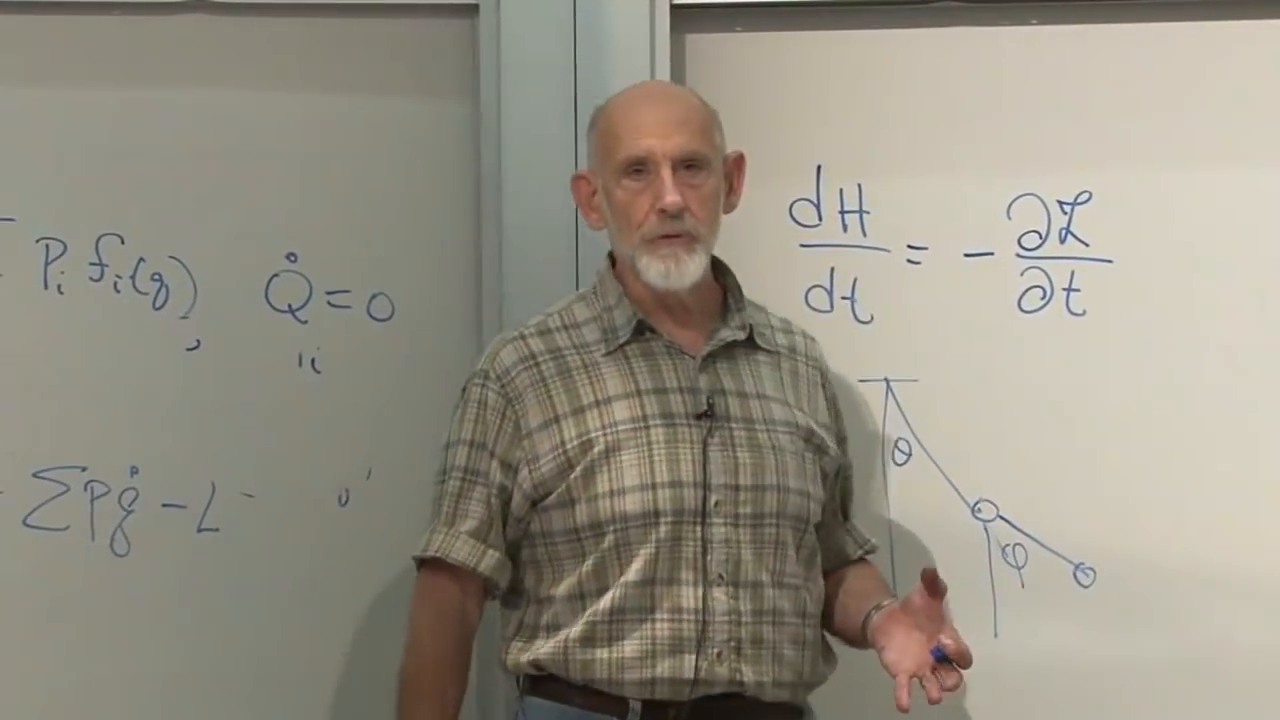
\includegraphics[width=0.84\textwidth]{lecture_05_figure_05.png}
  \caption{L’identité donnant le taux de variation de l’énergie reste au tableau à côté du
  schéma du double pendule.}
  \lectureframe{01:45:39}
\end{figure}

\begin{figure}[htbp]
  \centering
  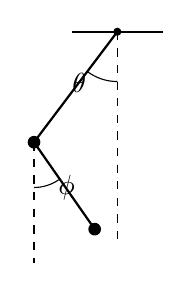
\begin{tikzpicture}[scale=1.15]
    \draw[thick] (-0.5,0) -- (0.5,0);
    \fill (0,0) circle (0.045);
    \draw[dashed] (0,0) -- (0,-2.3);
    \draw[thick] (0,0) -- (-0.92,-1.22);
    \fill (-0.92,-1.22) circle (0.07);
    \draw[dashed] (-0.92,-1.22) -- (-0.92,-2.55);
    \draw[thick] (-0.92,-1.22) -- (-0.25,-2.18);
    \fill (-0.25,-2.18) circle (0.07);
    \draw (0,-0.55) arc (-90:-127:0.55);
    \node at (-0.42,-0.56) {$\theta$};
    \draw (-0.92,-1.72) arc (-90:-55:0.48);
    \node at (-0.56,-1.72) {$\phi$};
  \end{tikzpicture}
  \caption{Coordonnées angulaires généralisées d’un double pendule.}
\end{figure}

Le changement de variables est tout aussi efficace : on transforme un lagrangien puis
on en déduit les équations, au lieu de transformer séparément chaque équation des forces.

\begin{classroomqa}
  \audiencequestion{Le pendule double est-il essentiellement un autre système à trois corps, comme le Soleil, la Terre et la Lune, où l’un des corps jouerait le rôle d’ancrage ?
  \lecturetimestamp{01:45:06--01:45:25}}
  \lecturerresponse{Cette analogie rend bien compte de la hiérarchie, même si les tiges imposent des contraintes différentes. Dans les deux cas, on peut, dans une approximation, traiter un composant très massif ou fixe comme structure de référence.}
\end{classroomqa}

\begin{classroomqa}
  \audiencequestion{Le pendule double utilise \(T-V\), alors que nous venons d’insister sur le fait que les lagrangiens peuvent être plus généraux. Dans quels cas \(T-V\) est-il valable ?
  \lecturetimestamp{01:46:08--01:46:58}}
  \lecturerresponse{Cette forme usuelle s’applique aux particules non relativistes ordinaires décrites dans un référentiel inertiel, en l’absence de couplage magnétique dépendant de la vitesse. Les référentiels en rotation, les systèmes relativistes et les champs magnétiques nécessitent des termes plus généraux.}
\end{classroomqa}

\begin{classroomqa}
  \audiencequestion{Les collisions échappent-elles à cette description ?
  \lecturetimestamp{01:47:00--01:48:05}}
  \lecturerresponse{Les collisions élastiques résultent de forces de courte portée et donc de potentiels. À l’échelle microscopique, les collisions inélastiques restent mécaniques, mais de l’énergie est transférée aux vibrations internes, à la déformation et à la chaleur. Une description du centre de masse qui omet ces degrés de liberté est incomplète.}
\end{classroomqa}

\begin{classroomqa}
  \audiencequestion{Peut-on analyser une balle de baseball frappée par une batte à l’aide de \(F=ma\) ?
  \lecturetimestamp{01:48:05--01:48:33}}
  \lecturerresponse{Seulement à un niveau approximatif. Une description complète doit prendre en compte la déformation, l’échauffement, les dommages éventuels à la balle et peut-être même la rupture de la batte. Ces degrés de liberté internes expliquent pourquoi un impact réaliste est bien plus difficile à décrire qu’une collision entre particules ponctuelles.}
\end{classroomqa}

\begin{classroomqa}
  \audiencequestion{Qu’en est-il d’un solide étendu ?
  \lecturetimestamp{01:48:34--01:49:00}}
  \lecturerresponse{On peut étudier les solides soit par les méthodes newtoniennes, soit à l’aide d’un lagrangien \(T-V\) écrit en coordonnées de translation et de rotation. Construire ce lagrangien est un exercice utile.}
\end{classroomqa}

\begin{classroomqa}
  \audiencequestion{La relation d’incertitude quantique entre l’énergie et le --temps signifie-t-elle que l’énergie n’est pas strictement conservée ?
  \lecturetimestamp{01:49:01--01:49:29}}
  \lecturerresponse{Non. L’énergie peut être strictement conservée. Cette relation signifie que déterminer l’énergie avec une grande précision exige une observation de longue durée ; elle ne remplace pas la loi de conservation.}
\end{classroomqa}

\begin{classroomqa}
  \audiencequestion{La mécanique newtonienne et la mécanique lagrangienne sont-elles logiquement équivalentes ?
  \lecturetimestamp{01:49:36--01:50:07}}
  \lecturerresponse{Elles sont équivalentes dans le domaine usuel où les deux formulations s’appliquent. On peut néanmoins inventer des lagrangiens dont les équations ne ressemblent pas à la forme élémentaire \(m\ddot x=F(x)\).}
\end{classroomqa}

\section{Un terme cinétique dépendant des coordonnées}

Considérons l’exemple volontairement peu familier
\begin{equation}
  L=\frac12q^2\dot q^2-\frac12q^2.
  \label{eq:l5-nonstandard-l}
\end{equation}
Il s’agit d’un lagrangien valide dont le coefficient cinétique dépend des coordonnées. On pourrait également considérer des termes linéaires en vitesse, tels que \(q\dot q\) ; dans cet exemple à une dimension, ce terme particulier est une dérivée totale et ne modifierait pas les équations du mouvement.

La quantité de mouvement canonique est
\begin{equation}
  p=\frac{\partial L}{\partial\dot q}=q^2\dot q,
  \label{eq:l5-nonstandard-p}
\end{equation}
donc
\begin{equation}
  \dot p=q^2\ddot q+2q\dot q^2,
  \qquad
  \frac{\partial L}{\partial q}=q\dot q^2-q.
  \label{eq:l5-nonstandard-derivatives}
\end{equation}
L’équation du mouvement est donc
\begin{equation}
  q^2\ddot q+q\dot q^2=-q.
  \label{eq:l5-nonstandard-eom}
\end{equation}

\begin{figure}[htbp]
  \centering
  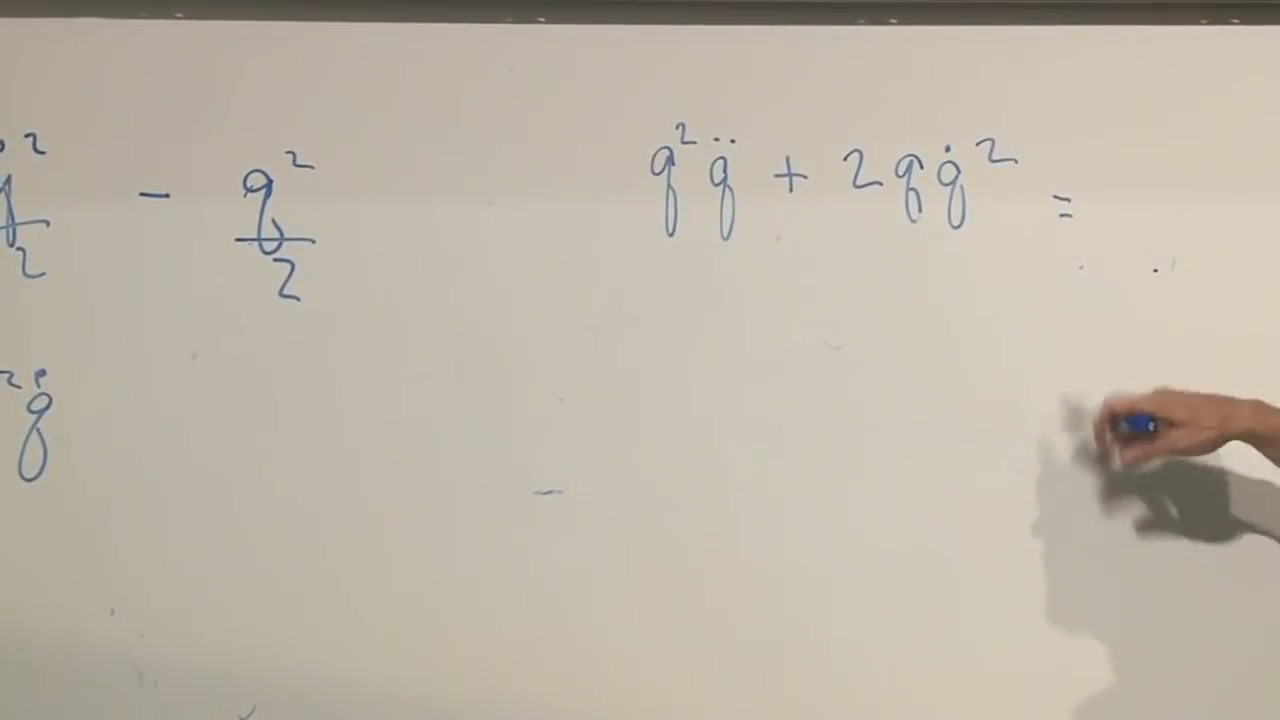
\includegraphics[width=0.80\textwidth]{lecture_05_figure_06.png}
  \caption{La quantité de mouvement dérivée dans l’exemple où le terme cinétique dépend des coordonnées.}
  \lectureframe{01:52:32}
\end{figure}

\begin{classroomqa}
  \audiencequestion{Peut-on diviser l’équation par \(q\) ?
  \lecturetimestamp{01:53:22--01:53:39}}
  \lecturerresponse{Seulement lorsque \(q\neq0\). Pour \(q=0\), le coefficient cinétique et l’application de Legendre sont dégénérés ; une division ferait donc disparaître un point singulier qui doit être traité séparément.}
\end{classroomqa}

Le hamiltonien est
\begin{align}
  H&=p\dot q-L
  \notag\\
   &=q^2\dot q^2-
     \left(\frac12q^2\dot q^2-\frac12q^2\right)
  \notag\\
   &=\frac12q^2\dot q^2+\frac12q^2.
  \label{eq:l5-nonstandard-h}
\end{align}

\begin{classroomqa}
  \audiencequestion{Peut-on encore appeler \(q^2\dot q^2/2\) l’énergie cinétique ?
  \lecturetimestamp{01:54:41--01:55:07}}
  \lecturerresponse{Oui. Dans cet exemple développé, le hamiltonien a de nouveau l’apparence d’un terme cinétique positif auquel s’ajoute un terme de potentiel. L’essentiel est que les définitions formelles ont fonctionné sans qu’il soit nécessaire de supposer au préalable la forme élémentaire à masse constante.}
\end{classroomqa}

\section{Dissipation et origine profonde du formalisme}

\begin{classroomqa}
  \audiencequestion{Comment inclure le frottement dans un lagrangien ?
  \lecturetimestamp{01:55:09--01:56:17}}
  \lecturerresponse{Pas comme force fondamentale dans le système fermé simple à nombre fini de degrés de liberté considéré ici. Le frottement macroscopique est un effet statistique dû à un très grand nombre de degrés de liberté microscopiques. Ces atomes obéissent toujours à la mécanique sous-jacente, mais une description réduite qui ne les suit pas fait apparaître une dissipation.}
\end{classroomqa}

\begin{classroomqa}
  \audiencequestion{Comment Hamilton est-il parvenu à sa formulation ?
  \lecturetimestamp{01:56:22--01:56:37}}
  \lecturerresponse{Aucune dérivation historique n’a été présentée ici. Pour le cours actuel, l’essentiel est de comprendre le fonctionnement de cette formulation.}
\end{classroomqa}

\begin{classroomqa}
  \audiencequestion{Existe-t-il une méthode plus générale pour obtenir un lagrangien lorsqu’il n’a pas manifestement la forme \(T-V\) ?
  \lecturetimestamp{01:56:43--01:58:54}}
  \lecturerresponse{L’expérience, une conjecture éclairée, un principe de symétrie ou la reconstruction à partir des équations souhaitées peuvent fournir la fonction. Demander au calcul lui-même d’où vient son entrée revient à demander à la définition d’une dérivée d’où vient \(f(x)\). Le calcul nous indique quoi faire une fois la fonction spécifiée. La mécanique quantique apporte, à un niveau plus profond, une réponse à la question de savoir pourquoi les systèmes fermés de la nature obéissent à cette structure abstraite.}
\end{classroomqa}

Ce point rejoint les thèmes abordés au début du cours. L’évolution hamiltonienne fondamentale est déterministe et réversible, en ce sens que les trajectoires ne fusionnent pas et que l’information n’est pas simplement détruite. Le lien entre cette propriété et la formulation dans l’espace des phases sera développé progressivement.

\begin{classroomqa}
  \audiencequestion{Le calcul variationnel s’est-il contenté de remonter à partir des équations classiques souhaitées, et la mécanique quantique obtient-elle son lagrangien de la même manière ?
  \lecturetimestamp{01:59:37--02:01:07}}
  \lecturerresponse{Dans la construction classique élémentaire, on peut effectivement choisir une action dont les trajectoires stationnaires reproduisent les équations connues. En mécanique quantique, l’ordre logique est différent : on part naturellement du hamiltonien pour aboutir à une description lagrangienne. Le hamiltonien y est plus intuitif, même s’il paraît d’abord abstrait en mécanique classique.}
\end{classroomqa}

\begin{classroomqa}
  \audiencequestion{La mécanique quantique peut-elle décrire le frottement ?
  \lecturetimestamp{02:01:08--02:02:05}}
  \lecturerresponse{Oui, mais une description fondamentale doit inclure les degrés de liberté de l’environnement. On ne peut décrire complètement une particule se déplaçant dans un fluide visqueux sans inclure les particules du fluide. Le frottement est l’effet collectif complexe qui émerge lorsque ces degrés de liberté ne sont pas suivis individuellement.}
\end{classroomqa}
